\section{R\'{e}sultats principaux}\label{sec:res}

\subsection{Notations}
Dans la th\`{e}se, le symbol $X$ d\'{e}signe une variable al\'{e}atoire ($\vec{X}$ pour un vecteur colonne al\'{e}atoire) sur un ensemble $\mathcal{X}$, et $x$ (respectivement $\vec{x}$) d\'{e}signe une r\'{e}alisation de $X$ (respectivement $\vec{X}$). 
La $i$-\`{e}me coordonn\'{e}e d'un vecteur $\vec{x}$ est indiqu\'{e}e par $\vec{x}[i]$, et le transpos\'{e} d'un vecteur $\vec{x}$ par $\vec{x}^\intercal$. Les matrices sont indiqu\'{e}es par des majuscules en gras, $\textbf{A}$ ou $\covmat$. Les traces acquises des canaux auxiliaires sont interpr\'{e}t\'{e}es comme r\'{e}alisations $\vLeakVec_1, \dots , \vLeakVec_N$ d'un vecteur al\'{e}atoire r\'{e}el $\vaLeakVec\in\mathbb{R}^\traceLength$, o\`{u} $\traceLength$ est la longueur du signal. Quand une m\'{e}thode de r\'{e}duction de dimension est utilis\'{e}e comme pr\'{e} traitement, celle-ci am\`{e}ne \`{a} la d\'{e}finition d'une fonction appel\'{e}e \emph{extracteur} et d\'{e}not\'{e} par $\extract \colon \mathbb{R}^\traceLength \rightarrow \mathbb{R}^\newTraceLength$. La variable sensible manipul\'{e}e pendant l'acquisition des traces est indiqu\'{e}e par $\sensRandVar$. Celle-ci peut avoir diff\'{e}rent formes, mais souvent dans cette th\`{e}se elle est d\'{e}finie comme $\sensRandVar = \sensFunction(\keyRandVar,\publicParRandVar)$, o\`{u} $\publicParRandVar$ d\'{e}note une variable publique, par exemple une partie de message en clair, et $\keyRandVar$ une partie d'une cl\'{e} secr\`{e}te que l'attaquante souhaite retrouver. Les valeurs acquises par la variable sensible sont vus comme r\'{e}alisation de la variable al\'{e}atoire $\sensRandVar$ en $\sensVarSet = \{\sensVarValue{1}, \dots, \sensVarValue{\nbClasses}\}$. Les \'{e}l\'{e}ments de $\sensRandVar$ sont parfois encod\'{e}s via le \emph{one-hot-encoding}: \`{a} chaque \'{e}l\'{e}ment $\sensVarValue{j}$ on associe un vecteur de dimension $\numClasses$ $\sensVarOneHot{j}$, avec toutes les entr\'{e}es nulles, sauf la $j$-\`{e}me qui est \'{e}gal \`{a}  $1$: $\sensVarValue{j}
\rightarrow \sensVarOneHot{j} = (0,\ldots , 0,\underbrace{1}_{j},0,\dots,0)$. Un \'{e}l\'{e}ment g\'{e}n\'{e}rique de $\sensVarSet$ sera indiqu\'{e} par $\sensVarGenValue$, si sp\'{e}cifier son indexe  $i$ n'est pas n\'{e}cessaire.

\subsection{Techniques Lin\'{e}aires de R\'{e}duction de Dimension}\label{sec:lin}
Dans cette section sont d\'{e}crites les \'{e}tudes men\'{e}es aux tour des m\'{e}thodes lin\'{e}aires d'extraction de caract\'{e}ristiques, en particulier de l'Analyse aux Composantes Principales (PCA) et de l'Analyse Discriminante Lin\'{e}aire (LDA). 
\subsubsection{Analyse aux Composantes Principales, l'outil classique et le profil\'{e}e}
L'extracteur lin\'{e}aire $\extract^{\mathrm{PCA}}(\vLeakVec) = \textbf{A}\vLeakVec$ se d\'{e}duit des certains vecteurs propres $\AAlpha_1, \dots, \AAlpha_\newTraceLength$, appel\'{e}s \emph{Composantes Principales} (PCs), dont les transpos\'{e}s sont arrang\'{e} en tant que lignes dans la matrice de projection $\textbf{A}$. Classiquement la PCA intervient sur des donn\'{e}es non labellis\'{e}es $\vLeakVec_1, \dots , \vLeakVec_N$, suppos\'{e} ayant moyenne nulle et arrang\'{e} comme colonnes dans une matrice  $\measuresMatrix$ de dimension $\traceLength \times \nbTraces$, de tel sort que la matrice de covariance des donn\'{e}es est la suivante:
\begin{equation}\label{eq:covmat}
\covmat = \frac{1}{\nbTraces}\measuresMatrix\measuresMatrix^\intercal \mbox{ .}
\end{equation}

Dans ce cas, les vecteur propres $\AAlpha_1, \dots, \AAlpha_\newTraceLength$ correspondent aux vecteurs propres de la matrice $\covmat$ et leur valeur propres associ\'{e}s sont d\'{e}not\'{e}s $\lambda_1, \dots, \lambda_r$. La PCA est la projection qui maximise la variance globale des caract\'{e}ristiques extraites. La variance \'{e}tant li\'{e}e \`{a} la quantit\'{e} d'information des donn\'{e}es, cette transformation est cens\'{e}e r\'{e}duire la dimension des traces tout en renforçant l'information contenue. Une propri\'{e}t\'{e} remarquable de la PCA est que chaque $\lambda_i$ correspond \`{a} la variance empirique des donn\'{e}es projet\'{e}es sur la PC correspondante $\AAlpha_i$.\\

Dans un sc\'{e}nario d'attaque profil\'{e}e, cette outil classique est toutefois largement sous-optimal: ce n'exploite pas une phase de caract\'{e}risation. Dans cette derni\`{e}re on suppose que l'attaquante est en possession d'un ensemble de donn\'{e}es labellis\'{e}es  $(\vLeakVec_i, \sensVar_i)_{i=1..\nbProfilingTraces}$, c'est-\`{a}-dire o\`{u} l'association \emph{trace-variable sensible} est connue. Dans la litt\'{e}rature SCA \cite{TAprincipal,choudaryefficient,choudary2014efficient,disassembler,Standaert2008} une version \emph{profil\'{e}e} de la PCA a \'{e}t\'{e} introduite. En introduisant les moyennes empiriques par classe
\begin{equation}\label{eq:mmmXclass}
\mmmXclass= \esperEst[\given{\vaLeakVec}{\sensRandVar = \sensVarGenValue}] = \frac{1}{\nbTracesPerClass}\sum_{i\colon \sensVar_i=\sensVarGenValue} \vLeakVec_i  \mbox{ ,}
\end{equation}
la PCA profil\'{e}e utilise la matrice des \emph{\'{e}carts inter-classes} suivante \`{a} la place de la matrice de covariance $\covmat$:
\begin{equation}\label{eq:SB}
\SB = \sum_{\sensVarGenValue\in\sensVarSet}\nbTracesPerClass(\mmmXclass-\mmmX)(\mmmXclass-\mmmX)^\intercal \mbox{ ,}
\end{equation}
o\`{u} $\mmmX$ est la moyenne empirique de toutes les donn\'{e}es confondues. L'extracteur obtenu en cette mani\`{e}re garanties que les centro\"ides par classes des donn\'{e}es projet\'{e}es sont \'{e}cart\'{e}s au maximum.


\subsubsection{L'enjeu du choix des composantes}\label{sec:ELV}
L'introduction de la PCA dans le contexte des SCA a levée les questions suivantes: \textit{combien} de composants et \textit{lesquelles} sont suffisantes/nécessaires pour réduire la dimension des traces sans perdre de l'information discriminante importante ? 
%
Une première réponse a été données dans \cite{choudary2014efficient}, en relation au concept de \emph{variance expliquée} (ou \emph{variance expliquée globale}, EGV) d'une PC $\AAlpha_i$:

\begin{equation}\label{eq:EGV}
\mathrm{EGV}(\AAlpha_i) =  \frac{\lambda_i}{\sum_{k=1}^r\lambda_k} \mbox{ .}
\end{equation}
Par définition, la somme de toutes les EGV est égal à $1$. Le choix des composantes basé sur le EGV consiste à fixer une valeur souhaité pour la \emph{variance expliquée cumulative} $\beta$ et à garder $\newTraceLength$ PCs distinctes, où $\newTraceLength$ est l'entier minimum tel que: 
\begin{equation}
\mbox{EGV}(\AAlpha_1) +\mbox{EGV}(\AAlpha_2) + \dots +\mbox{EGV}(\AAlpha_\newTraceLength) \geq \beta \mbox{  .}
\end{equation}
Si l'attaquant e une contrainte pour la dimension $\newTraceLength$, le choix par EGV consiste simplement à garder les $\newTraceLength$ premières composantes, dans l'ordre naturel des valeurs propres associées. Dans le contexte des SCA, ce type de choix ne semble pas être systématiquement le meilleur: des articles déclarent que les composantes leaders contiennent la plus grande quantité d'information, alors que d'autres suggèrent de défausser ces premières composantes \cite{Batina2012,specht}. 
% An example of this behaviour is provided in Fig.~\ref{fig:DPAcontest}. It may be noticed that the first component (plotted on the left) has high coefficients spread over the whole trace, while the sixth one  (on the right) has high coefficients localised in a small time interval, very likely to signalize the instants in which the target sensitive variable leaks.
%
%\begin{figure}
%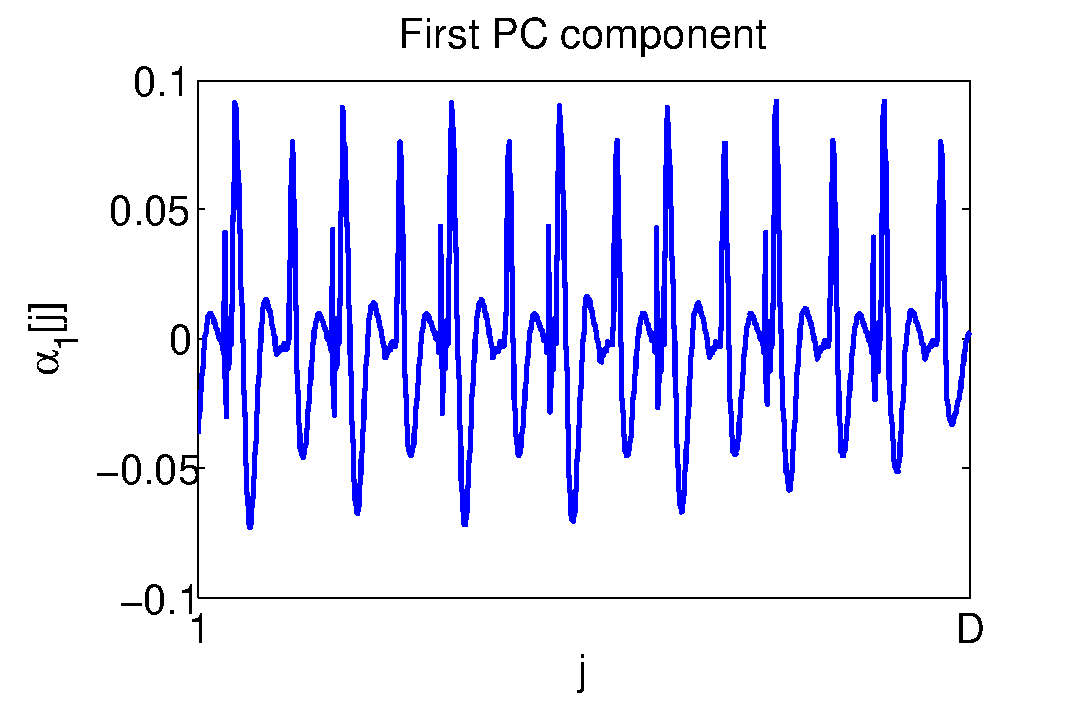
\includegraphics[width=.45\textwidth]{figures/DPAcontestPC1_new.pdf} 
%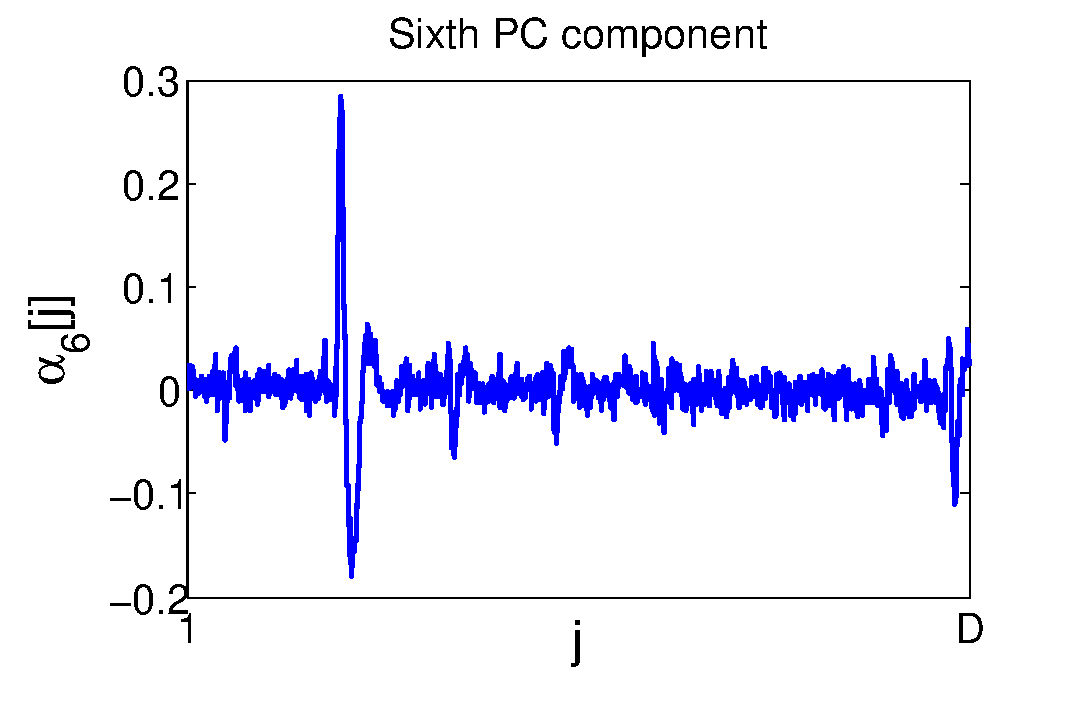
\includegraphics[width=.45\textwidth]{figures/DPAcontestPC6_new.pdf} 
%\caption{First and sixth PCs in DPA contest v4 trace set (between time samples 198001 and 199000)}\label{fig:DPAcontest}
%\end{figure}
%
Dans le contexte des implémentations sécurisées, le but des développeurs est de minimiser les fuites, autrement dit, de réduire le nombre de points de fuite, d'où l'assomption suivante qui peut être raisonnablement faite: 

\begin{assumption}\label{assum:local}
L'information compromettante d'une trace acquis de canaux auxiliaires est localisée en peu de points. 
\end{assumption}
Sous cette assomption, les auteurs de \cite{SCAclassProbl} ont donné donnée une deuxième réponse au problème du choix des composantes: ils utilisent le \emph{ratio de participation inversé} (IPR) pour évaluer la \emph{localisation} des vecteurs propres. Le IPR est ainsi défini:
\begin{equation}
\mathrm{IPR}(\AAlpha_i) = \sum_{j=1}^\traceLength \AAlpha_i[j]^4 \mbox{ .}
\end{equation}
Les auteurs de \cite{SCAclassProbl} suggèrent de sélectionner les PCs en ordre inverse par rapport à leur IPR. \\

%
\subsubsection{La méthode par variance expliquée locale} 
\begin{figure}
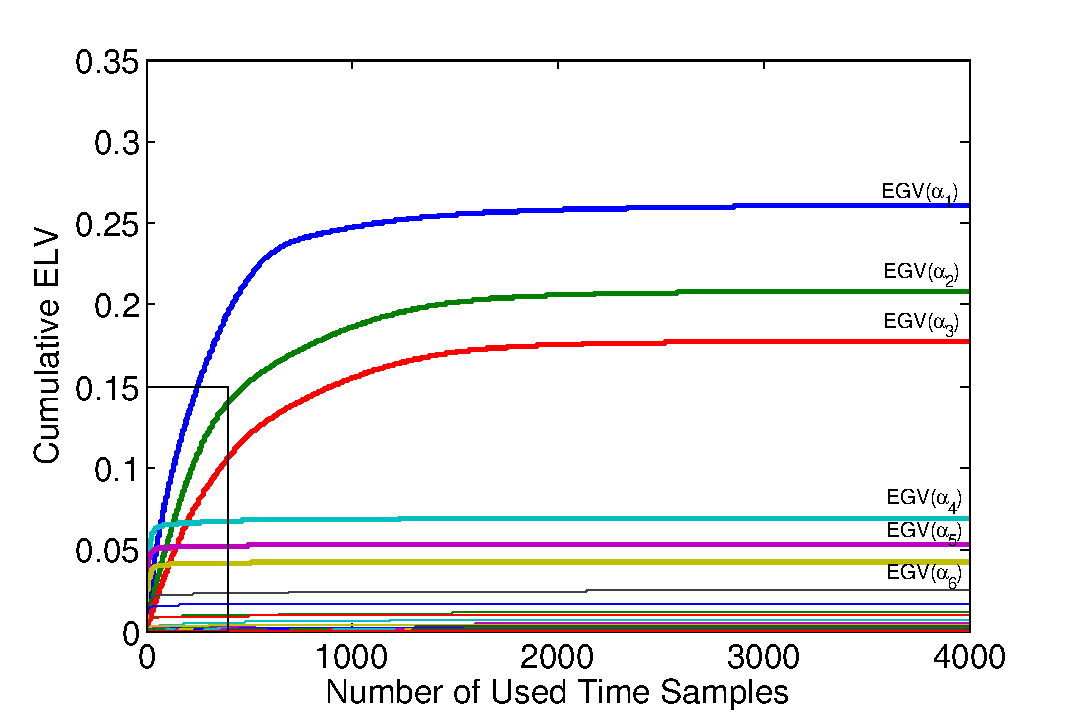
\includegraphics[width=0.5\textwidth]{figures/cumulativeELVallRectangle.pdf} 
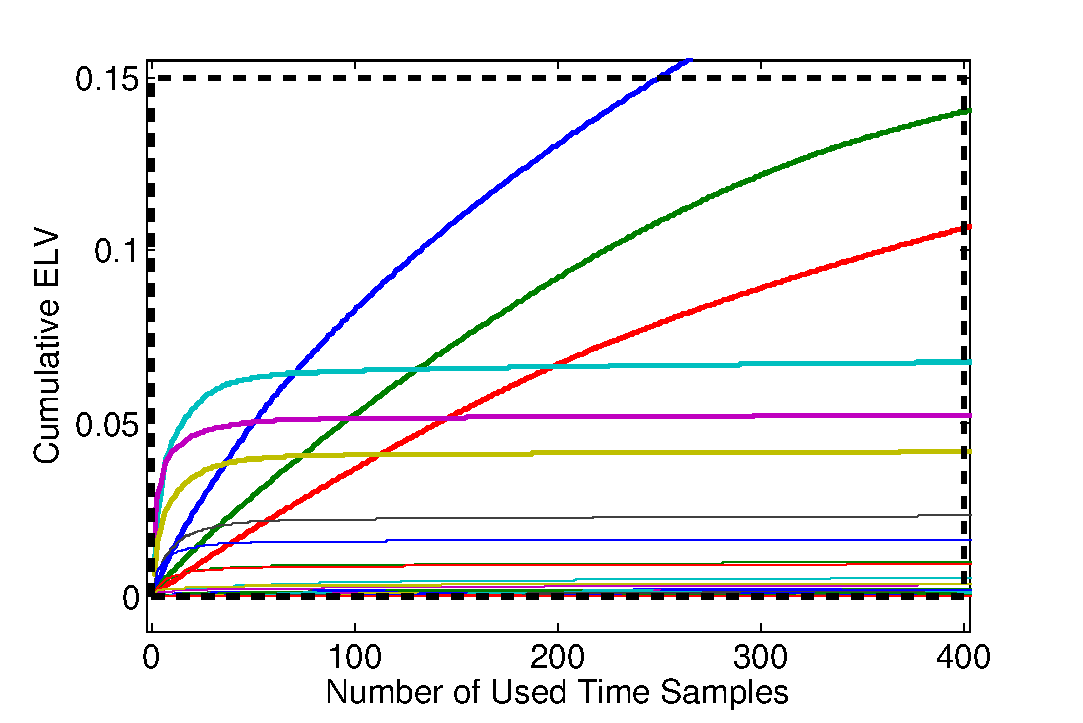
\includegraphics[width=0.5\textwidth]{figures/cumulativeELVzoomedRectangle.pdf} 
\caption{Cumulative ELV trend of principal components. On the right a zoom of the plot on the left. Acquisition campaign on an 8-bit AVR Atmega328P.}\label{fig:ELVcumulative}
\end{figure}
%
Les méthodes de sélection par EGV et IPR sont d'une certaine façon complémentaires : la première se base uniquement sur les valeurs propres associées aux PC et ne considère pas la forme des PC elles-mêmes; la seconde ne considère pas l'information donnée pas le valeurs propres, mais seulement la distribution des coefficients des PCs. Dans ce panorama nous avons proposé une nouvelle méthode se sélection qui fait un pont entre la EGV et la IPR : nous avons introduit la \emph{variance expliquée locale} (ELV) d'une PC $\AAlpha_i$ en un point $j$, définie par:
\begin{equation}
\mathrm{ELV}(\AAlpha_i,j) = \frac{\lambda_i \AAlpha_i[j]^2}{\sum_{k=1}^r\lambda_k} = \mathrm{EGV}(\AAlpha_i) \AAlpha_i[j]^2  \mbox{ .}
\end{equation}
Soit $\mathcal{J}=\{j^i_1, j^i_2, \dots, j^i_{\traceLength}\}\subset\{1,2,\dots,\traceLength\}$  un ensemble  d'indices ordonnés de tel sort que $\mathrm{ELV}(\AAlpha_i,j^i_1)\geq \mathrm{ELV}(\AAlpha_i,j^i_2)\geq \dots \geq \mathrm{ELV}(\AAlpha_i,j^i_\traceLength)$. On observe que la somme sur tous les $\mathrm{ELV}(\AAlpha_i,j)$, pour tout $j\in[1,\dots,\traceLength],$  est égal à $\mathrm{EGV}(\AAlpha_i)$. Si on opère cette somme en manière cumulative en suivant l'ordre donnée par l'ensemble ordonné $\mathcal{J}$, on obtient une description complète de la tendance suivie par la composante $\AAlpha_i$ pour atteindre son EGV. Comme montré in Fig.~\ref{fig:ELVcumulative}, où ces ELV cumulatives sont représentées, les trois premières composantes atteignent leur EGV finale très lentement, alors que la $4$ème, $5$ème et $6$ème atteignent une large partie de leur EGV très rapidement, c'est-à-dire an sommant les contributions ELV d'une moindre nombre de points. La sélection par ELV, en analogie avec EGV, demande de fixer une taille pour la dimension réduite du signal $\newTraceLength$, ou une seuil $\beta$ pour la ELV cumulative. Dans le premier cas les valeurs maximales de ELV de chaque PC sont comparées, et les $\newTraceLength$ montantes les valeurs plus élevées sont sélectionnées. Dans le second cas, tous les couple (PC, point temporel) sont ordonnés en ordre décroissant de ELV, et sommés jusqu'à atteindre le seuil $\beta$. Les PC qui contribuent à la somme sont sélectionnées.\\




\subsubsection{LDA et le probl\`{e}me de la taille de l'\'{e}chantillonnage}
L'extracteur $\extract^{\mathrm{LDA}}$ est une réduction de dimension optimale, sous certaines conditions, pour résoudre un problème de classification, c'est-à-dire un problème d'apprentissage où l'on vise à assigner à une donnée (une trace dans notre cas) un label (donné ici par la valeur de la variable $\sensRandVar$ manipulée lors de l'acquisition). Il a pour but non seulement d'écarter les centro\"ides par classe, mais aussi de reprocher au mieux les données appartenant à une même classe. La forte analogie entre les SCA et la tâche de classification en apprentissage automatique rend la LDA beaucoup plus adaptée 

%The   extractor $\extract^{\mathrm{LDA}}$ aims not only to spread class-centroids apart, but also to make data belonging to a same class as close as possible. As widely discussed in the literature \cite{Cagli2016,disassembler,Standaert2008}, the LDA method is more expensive than the PCA but more efficient. As for the PCA, the construction of the matrix $A$ is done through that of some eigenvectors, called in this case \emph{Linear Discriminant Components} (LDCs), which correspond to those of the matrix $\SW^{-1} \SB$, where $\SB$ is defined as in \eqref{eq:SB} and $\SW$ is known as the \emph{within-class scatter matrix}:
%
%\begin{equation}
%\SW = \sum_{\sensVar\in\sensVarSet}\sum_{i:z_i=z}(\sss[z_i]{i}-\mmmXclass)(\sss[z_i]{i}-\mmmXclass)^\intercal \mbox{.}
%\end{equation}
%
%The main drawback of the LDA, known as the {\em Small Sample Size problem} (SSS for short) occurs when the total number of acquisitions $\numTraces[]$ is less than or equal to the size $\traceLength$ of them, implying that the matrix $\SW$ is non-invertible. If the LDA has been introduced relatively lately in the SCA literature, the Pattern Recognition community looks for a solution to the SSS problem since the early nineties. I browsed some of the proposed solutions, testing some of them over side channel traces.
%
%\subsubsection{Results and conclusions}
%\begin{figure}[t]
%\subfigure[]{\label{fig:1.1}
%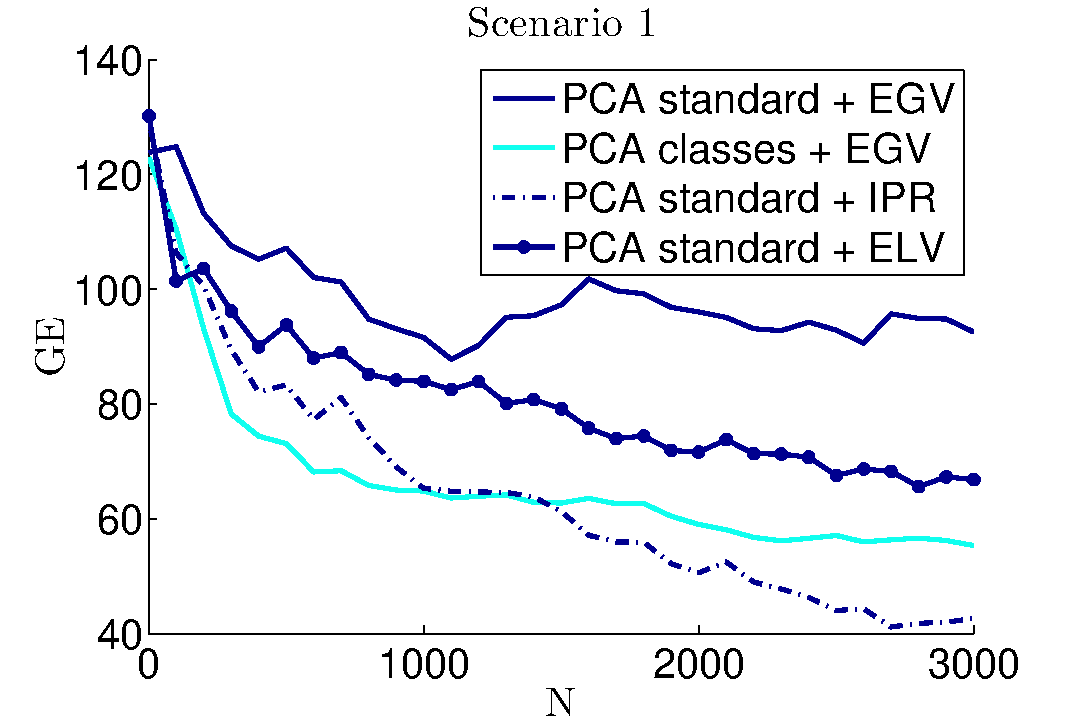
\includegraphics[width=0.5\textwidth]{figures/Criterion1.pdf}}
%\subfigure[]{\label{fig:1.2}
%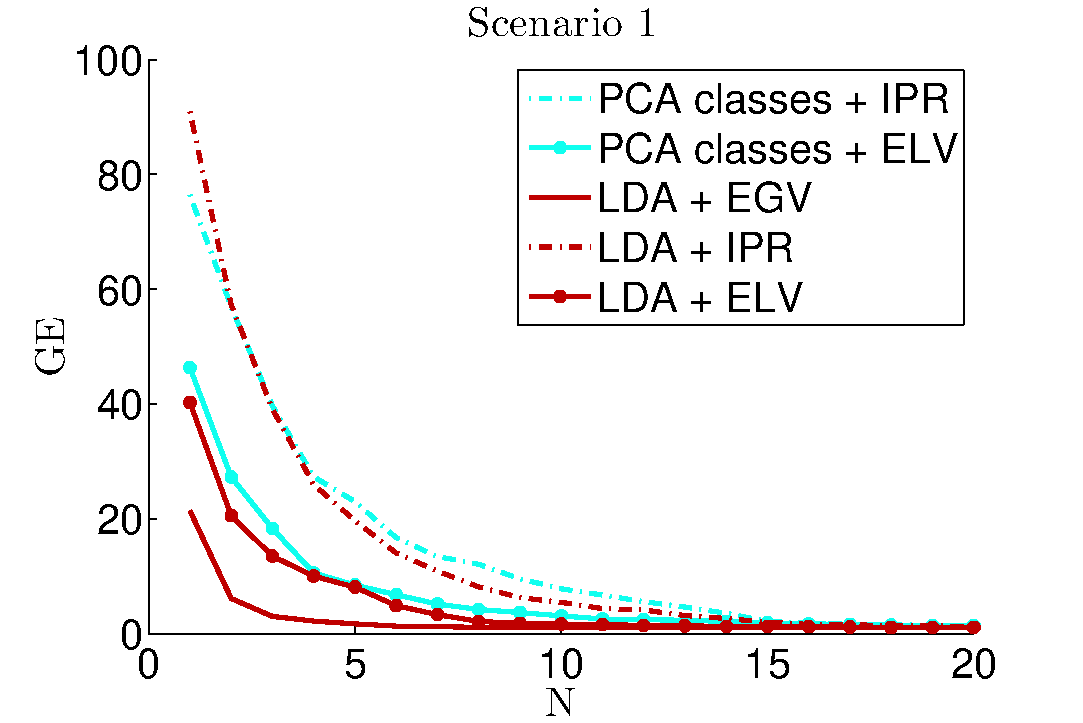
\includegraphics[width=0.5\textwidth]{figures/Criterion1Good.pdf}}
%\caption{Guessing Entropy (average rank of the right key hypothesis) as function of the number of attack traces for different extraction methods. All Guessing Entropies are estimated as the average rank of the right key over 100 independent experiments.}\label{fig:scenario1}
%\end{figure}
%
%\begin{figure}
%\subfigure[]{\label{fig:direct_PCA}
%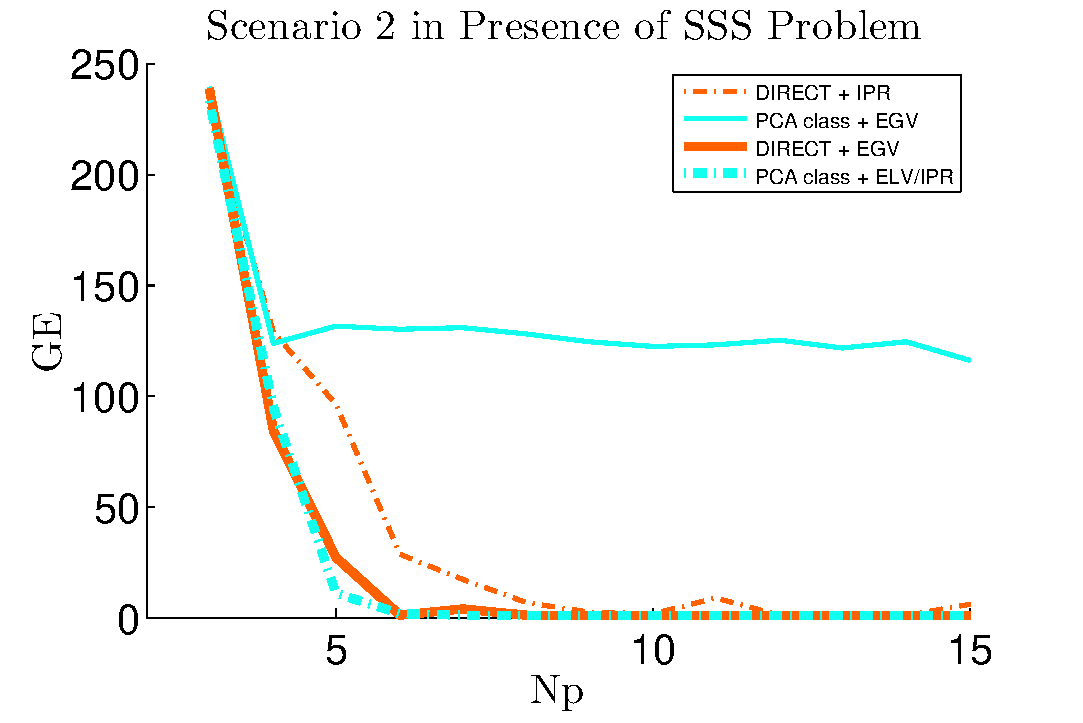
\includegraphics[width=0.5\textwidth]{figures/SSS.pdf}}
%\subfigure[]{\label{fig:notSSS}
%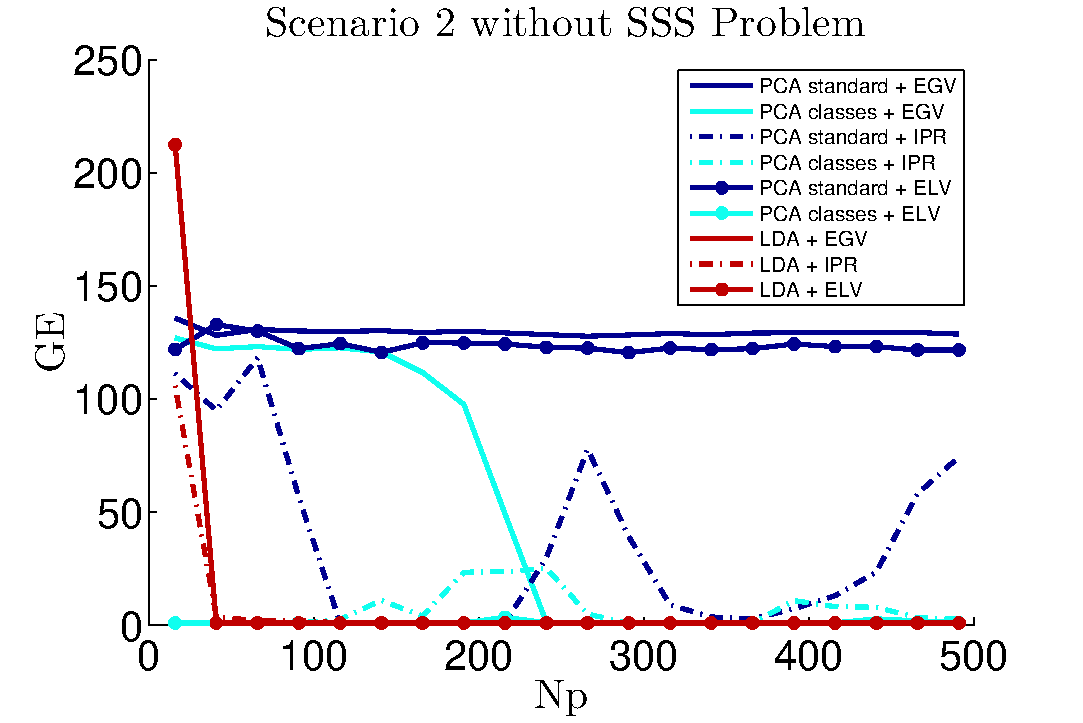
\includegraphics[width=0.5\textwidth]{figures/Criterion2notSSS.pdf}}
%\caption{Guessing Entropy as function of the number of profiling traces. Figure \subref{fig:direct_PCA} the best method extending the LDA and class-oriented PCA in presence of SSS problem; Figure \subref{fig:notSSS}: a comparison in absence of the SSS problem.}\label{fig:scenario2}
%\end{figure}
%
%Several experimental analyses have been performed in order to evaluate the ELV component selection technique and the techniques alternative to the LDA in presence of the SSS problem. In this section the most significant results are reported. They come out from two different scenarios: in the first one (Scenario 1) the attacker has a large number of profiling traces (denoted $N_p$) and wants to minimize the number of attack traces ($N_a$) to obtain a successful attack. Observing Fig.~\ref{fig:scenario1} three conclusions can be drawn: 
%\begin{itemize}
%\item the fact that the classical PCA (PCA standard) is largely suboptimal in a profiling context is validated
%\item the fact that the LDA technique is the most appropriate one is also validated
%\item equipping the class-oriented PCA with the ELV selection method (instead of the EGV one) significantly raises its performances, making them close to those of the LDA.
%\end{itemize}
%In the Scenario 2, the attacker aims instead to minimize the number of profiling traces ($N_p$) necessary to obtain a good extraction. In this case the SSS problem might occur. Observing Fig.~\ref{fig:scenario2} we conclude again that both in presence of not of the SSS problem, the PCA equipped with the ELV selection has performances close to those of the LDA or of its best alternative in presence of the SSS problem, called Direct LDA. 


\subsection{Analyse Discriminante par Noyau}\label{sec:kda}

%When a $(d-1)$th-order sharing is applied, the target $Z$ is represented by a $d$-tuple of shares $M_i$ manipulated at different times  $t_1,\dots,t_d$, and the sensitive information lies in the statistic $\esper[\SSS[]{}[t_1]\SSS[]{}[t_2]\cdots \SSS[]{}[t_d]]$, sometimes referred to as \emph{$d$-th order statistical moments}, meaning that the function\\ $f(z) = \esper[\SSS[]{}[t_1]\SSS[]{}[t_2]\cdots \SSS[]{}[t_d]\vert Z=z]$  is not constant. To exploit such information it has been shown  \cite{carlet2014achieving} that the statistic extracted from measurements, viewed as a multivariate polynomial in the time samples coordinates, must contain the $d$th-degree monomial $\prod_{i=1,\dots,d}\SSS[]{}[t_i]$.
%
%Since in practice the time samples $t_1,\dots,t_d$ are not known by the attacker, and even not unique, a good but naive idea to get an effective extractor is to look for linear combinations of the products of all possible $d$-tuples of points. It means immersing, via a non-linear function $\Phi$, the observed data in the higher-dimensional space $\featureSpace = \mathbb{R}^{D\choose{d}}$, and then look for a linear extractor (with PCA of LDA techniques, for example). The combinatorially explosion of the size of $\featureSpace$ is an obstacle from a computationally standpoint, since it requires the computation, storage and managements of ${D\choose{d}}$-sized traces.  The KDA algorithm enables an attacker to compute the LDA extractor over $\featureSpace$ without requiring computations into such a feature space, as depicted in Fig.~\ref{fig:scheme2}.\\
%
%The central tool of a kernel trick is the \emph{kernel function} $K \colon \mathbb{R}^\traceLength \times \mathbb{R}^\traceLength \rightarrow \mathbb{R}$, that has to satisfy the following property, in relation with the function $\Phi$:
%
%\begin{equation}\label{eq:kernelProperty}
%K(\sss[]{i},\sss[]{j}) = \Phi(\sss[]{i})\cdot \Phi(\sss[]{j}) \mbox{ ,}
%\end{equation}
%for each $i,j= 1,\dots, \NPoI$, where $\cdot$ denote the dot product.
%
%Every map $\Phi$ has an associated kernel function given by \eqref{eq:kernelProperty}, for a given set of data. The converse is not true: all and only the functions $K\colon\mathbb{R}^D\times \mathbb{R}^D \rightarrow \mathbb{R}$ that satisfy a convergence condition known as {\em Mercer's condition} are associated to some map $\Phi:\mathbb{R}^D	\rightarrow \mathbb{R}^F$, for some $F$. Importantly, a kernel function is interesting only if it is computable directly from the rough data $\sss[]{i}$, without evaluating the function $\Phi$. \\
%
%The notion of kernel function is illustrated in the following example.
%
%\begin{example}\label{ex:polyKernel}
%Let $D=2$. Consider the function
%\begin{align}
%&K\colon\mathbb{R}^2\times \mathbb{R}^2 \rightarrow \mathbb{R} \nonumber \\ 
%&K\colon(\sss[]{i},\sss[]{j}) \mapsto ( \sss[]{i}\cdot \sss[]{j})^2 \mbox{ ,} \label{eq:example1}
%\end{align}
%
%After defining $\sss[]{i} = [a,b]$ and $\sss[]{j} = [c,d]$, we get the following development of K:
%\begin{equation}
%K(\sss[]{i},\sss[]{j}) = (ac + bd)^2 = a^2c^2 + 2abcd + b^2d^2 \mbox{ ,}
%\end{equation}
%
%which is associated to the following map from $\Bbb{R}^2$ to $\Bbb{R}^3$:
%
%\begin{equation}
%\Phi(u,v) =  [u^2, \sqrt{2}uv, v^2]
%\end{equation}
%
%Indeed $\Phi(\sss[]{i})\cdot \Phi(\sss[]{j}) = a^2c^2 + 2abcd + b^2d^2 = K(\sss[]{i},\sss[]{j})$\enspace. This means that to compute the dot product between some data mapped into the $3$-dimensional space $\featureSpace$ there is no need to apply $\Phi$: applying $K$ over the $2$-dimensional space is equivalent. 
%
%\end{example}
%
%
%\begin{figure}
%\centering
%{
%\begin{tikzpicture}
%\matrix (m) [matrix of math nodes, row sep=3em,
%column sep=3em, text height=1.5ex, text depth=0.25ex]
%{ \mathbb{R}^\traceLength & \featureSpace & \mathbb{R}^\newTraceLength \\};
%\path[->]
%(m-1-1) edge node[above] {$\Phi$} (m-1-2);
%         %edge [bend left=30] (m-2-2)
%         %edge [bend right=15] (m-2-2);
%\path[->]
%($(m-1-2.north east)-(0,0.1)$) edge node[above] {$\extract^{\mathrm{PCA}}$} ($(m-1-3.north west)-(0,0.1)$);
%\path[->]
%($(m-1-2.south east)+(0,0.15)$) edge node[below] {$\extract^{\mathrm{LDA}}$} ($(m-1-3.south west)+(0,0.15)$);
%
%\path[->]
%(m-1-1) edge [bend left=50] node[above] {$\extract^{\mathrm{KPCA}}$} (m-1-3)
%(m-1-1) edge [bend right=50] node[below] {$\extract^{\mathrm{KDA}}$} (m-1-3);
%
%\end{tikzpicture} 
%}
%\caption{Applying KDA and KPCA permits to by-pass computations in $\featureSpace$.}\label{fig:scheme2}
%\end{figure}
%
%
%The function $K(\sss[]{i},\sss[]{j}) = (\sss[]{i} \cdot \sss[]{j})^d$, hereafter named \emph{$d$th-degree polynomial kernel function}, is the convenient choice for an attack against implementations protected with $(d-1)$th-order masking: it corresponds to a function $\Phi$ that brings the input coordinates into a feature space $\featureSpace$ containing all possible $d$-degree monomials in the coordinates of $\sss[]{}$, up to constants. This is, up to constants, exactly the $\Phi$ function of Fig.~\ref{fig:scheme2}. The KDA methodology is described in the following procedure.
%
%\subsubsection*{Procedure: KDA for $d$th-order masked side-channel traces}\label{procedure:KDA}
%Given a set of labelled side-channel traces $(\sss[z_i]{i})_{i=1,\dots,\NPoI}$ and the kernel function $K(\sss[]{},\yyy)= (\sss[]{}\cdot \yyy)^d$:
%\begin{itemize}
%\item[1)] Construct a matrix $\MMM$ (acting as \emph{between-class scatter matrix}):
%
%\begin{equation}
%\MMM = \sum_{\sensVar\in\sensVarSet}\numTraces(\MMMclass - \MMMT)(\MMMclass-\MMMT)^\intercal\mbox{ ,}
%\end{equation}
%
%where $\MMMclass$ and $\MMMT$ are two $N$-size column vectors whose entries are given by:
%\begin{align}
%\MMMclass[z][j] = \frac{1}{\numTraces}\sum_{i:z_i=z}^{\numTraces}K(\sss[z_j]{j},\sss[z_i]{i})\\
%\MMMT[j] = \frac{1}{\NPoI}\sum_{i=1}^{\NPoI}K(\sss[z_j]{j},\sss[z_i]{i}) \mbox{ .}
%\end{align}
%
%
%\item[2)] Construct a matrix $\NNN$ (acting as \emph{within-class scatter matrix}):
%
%\begin{equation}\label{eq:N}
%\NNN = \sum_{\sensVar\in\sensVarSet}\kernelMatrix_\sensVar(\III - \III_{\numTraces)}\kernelMatrix_\sensVar^\intercal\mbox{ ,}
%\end{equation}
%where $\III$ is a $\numTraces\times \numTraces$ identity matrix, $\III_{\numTraces}$ is a $\numTraces\times \numTraces$ matrix with all entries equal to $\frac{1}{\numTraces}$ and $\kernelMatrix_{\sensVar}$ is the $\NPoI\times \numTraces$ sub-matrix of $\kernelMatrix = (K(\sss[z_i]{i},\sss[z_j]{j}))_{\substack{i=1,\dots,\numTraces[] \\ j=1,\dots,\numTraces[]}}$ storing only columns indexed by the indices $i$ such that $z_i=z$. 
%
%
%\item[2bis)] Regularize the  matrix $\NNN$ for computational stability:
%\begin{equation}\label{eq:mu}
%\NNN = \NNN + \mu  \III 
%\end{equation}
%
%\item[3)]\label{point:eigs} Find the non-zero eigenvalues $\lambda_1, \dots, \lambda_\numEigenvectors$ and the corresponding eigenvectors $\nununu_1, \dots, \nununu_\numEigenvectors$ of $\NNN^{-1}\MMM$; 
%
%
%\item[4)] Finally, the projection of a new trace $\sss[]{}$ over the $\ell$-th non-linear $d$-th order discriminant component can be computed as:
%\begin{equation}\label{eq:projection}
%\extract^{\mathrm{KDA}}_{\ell}(\vec{x}) = \sum_{i=1}^{\NPoI}\boldsymbol{\nu}_\ell[i]K(\sss[z_i]{i}, \sss[]{}) \mbox{ .}
%\end{equation} 
%
%\end{itemize}
%
%\subsubsection{Analysis and results}
%\begin{figure}[t]
%\subfigure[]{\label{fig:numClasses-2order}
%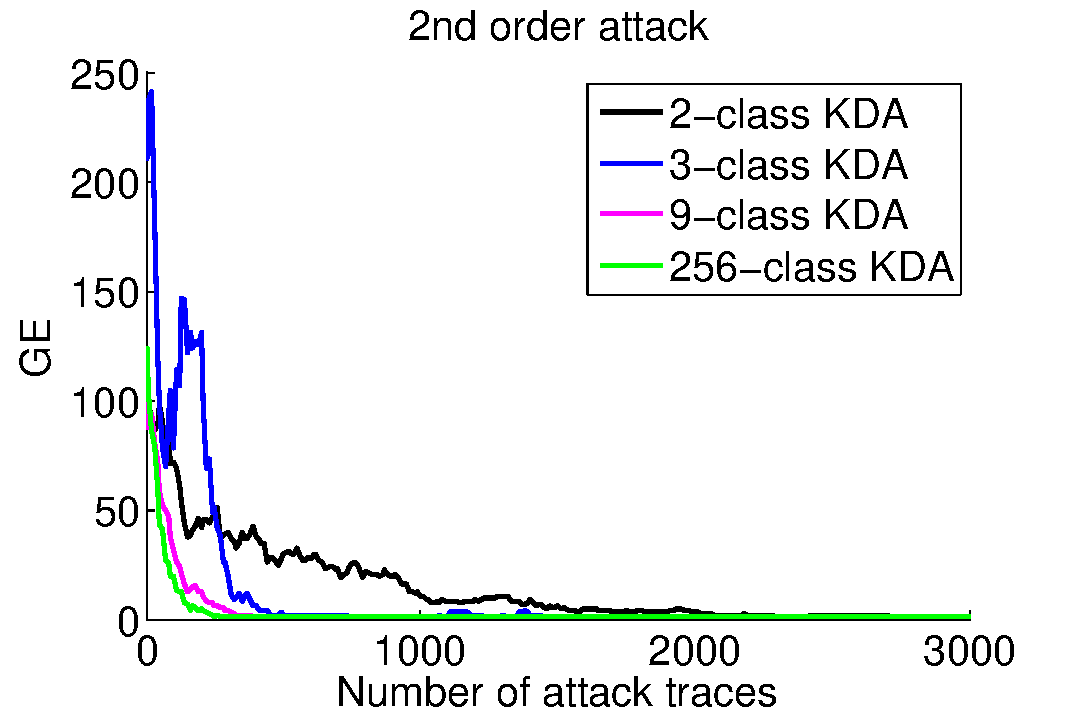
\includegraphics[width=.5\textwidth]{figures/2order_classes_TA.pdf}}
%\subfigure[]{\label{fig:numClasses-3order}
%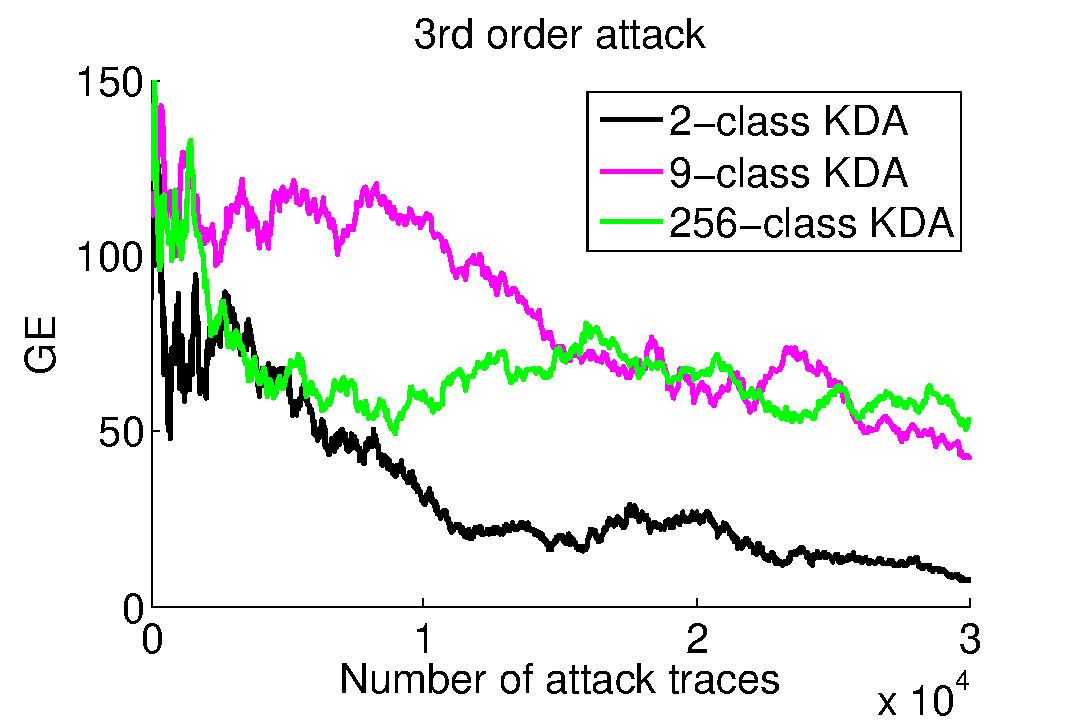
\includegraphics[width=.5\textwidth]{figures/3order_new.pdf}}
%\caption{Comparison between 2-class, 3-class, 9-class and 256-class KDA in $2$nd-order context \subref{fig:numClasses-2order} and in $3$rd-order context \subref{fig:numClasses-3order}. For $2$nd-order the KDA is efficient in providing separability between 256 classes, allowing an optimal attack. In $3$rd-order context the training data are not enough to succeed the 256-class learning phase. Decreasing the number of classes to be distinguished raises the efficiency of the learning problem and thus of the attack.}\label{fig:numClasses}
%\end{figure}
%
%The first aspect of the application of the KDA I focused on is the importance of a good regularization (provided by the choice of the parameter  $\mu$ in \eqref{eq:N}): it is an answer to the fact that kernel methods are generally prone to over-fitting: this means, in the case of the KDA, that $\extract^{\mathrm{KDA}}$ risks to perfectly separate the training traces in their classes, while failing in separating the attack traces. The regularization acts as an additional constraint of the problem, that makes the method less accurate in the learning phase, but in some cases more likely to correctly operate on new examples. I observed that extractors issued by a well-regularized KDA were localised over few $d$-tuples of points, and this property was again (as for linear extractors) sign of a good underlying detection of the informative PoIs. \\
%
%A second aspect I focused on is the role of the target model in the accuracy-efficiency trade-off. Since the complexity of the KDA is $O(N^3)$, where $N$ is the total number of training traces, it may be interesting to minimize such a $N$ in order to raise the efficiency of the computation. Nevertheless, bounding $N$ reduces the accuracy of the KDA. A way to alleviate this loss of accuracy is to reduce at the same time the number of classes to separate: a non-injective model $m(\cdot)$ can be introduced, to create a smaller set of labels $m(\sensVarSet)$ from the initial set $\sensVarSet$. For example, different values of $Z$ may be grouped according to their Hamming weights: a $2$-class model may be given by ($m(z) =0$ if $\HW(z)<4$, $m(z) =1$ if $\HW(z)\geq4$). Once a model $m(\cdot)$ is chosen and a KDA preprocessing based on such a model has been performed, it seems more adequate to run an attack based on the same target model $m(\cdot)$ (characterizing $\lvert m(\sensVarSet)\rvert$ different signals). Fixing the number $N$ of training traces, the results of this kind of attacks are depicted in Fig.~\ref{fig:numClasses}: if in $2$nd-order context it can be observed that the KDA is provided with sufficient training traces to succeed a 256-class separation, moving to the $3$-rd order context the conversion to a 2-class problem turns out to be a good strategy.
%
%\begin{figure}
%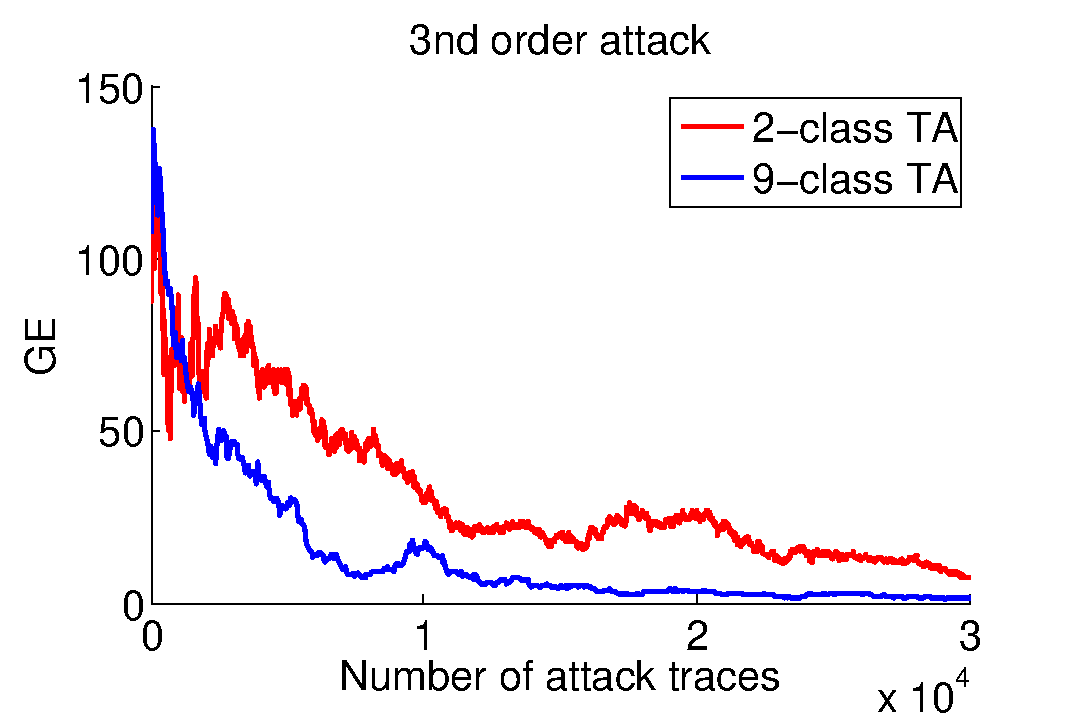
\includegraphics[width=.5\textwidth]{figures/3order_2_9.pdf} 
%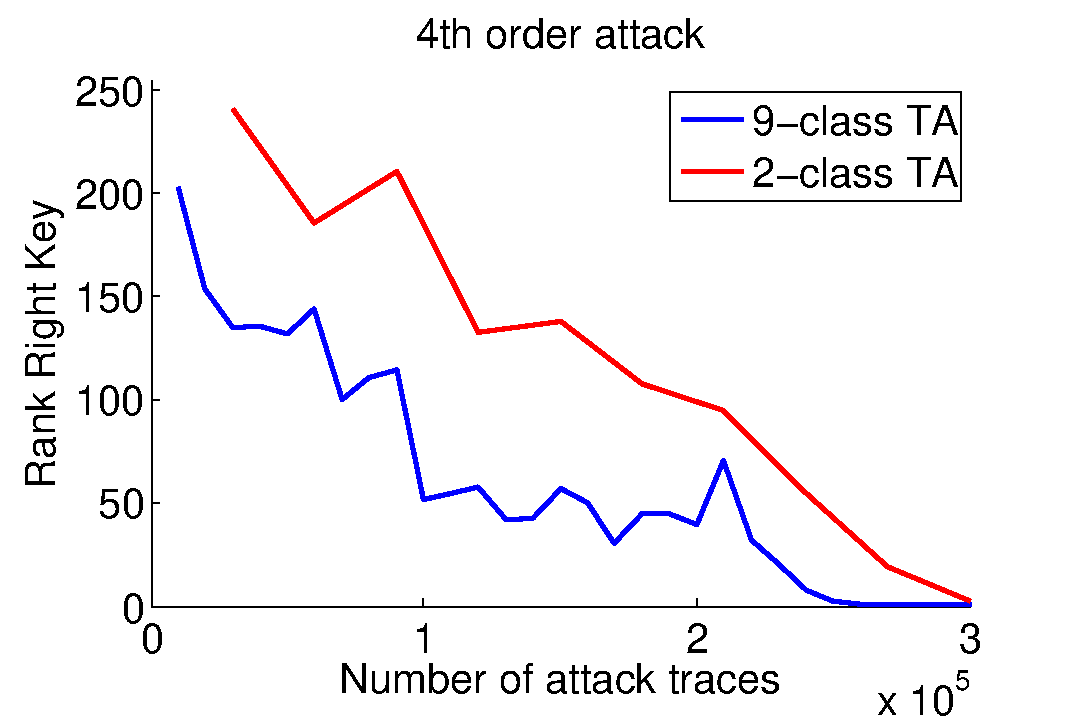
\includegraphics[width=.5\textwidth]{figures/4order_2_9.pdf} 
%\caption{Left: guessing entropy  for a 2-class and a 9-class $3$rd-order template attack. Right: right key rank of a 2-class and a 9-class $4$th-order template attack.}\label{fig:3-4}
%\end{figure}
%
%Third, I evaluated the soundness of an asymmetric preprocessing-attack approach. The success of a 2-class extractor always relies on a good exploitation of the PoIs, whose position does not depend on the chosen target model. For this reason, even if an extractor has been trained to separate $W$ classes, it does not mean that a finest characterization is useless. Results depicted in Fig.~\ref{fig:3-4} come from this asymmetric approach: the extractors used have been trained over $2$ classes, but the attacks that exploit a $9$-class characterization are more efficient.  
%
%Finally, I effectuated a comparison between the KDA and the PP approach. In particular I compared their performances under a fixed training set size, concluding that the effectiveness of the KDA is much less affected by the increase of the order $d$ than the PP. Indeed, the latter failed the PoI detection at orders 3 and 4.


\subsection{R\'{e}seau Neuronal Convolutif}\label{sec:cnn}